
\documentclass[12pt]{letter}

\usepackage[margin=1in,footskip=0.25in]{geometry}
\usepackage{tikz-cd}
\usetikzlibrary{positioning} % for the original

\begin{document}
Viet Tran Quoc Hoang \\ ID: 01607460 \\  09/23/2017 \\ COMP 3040 : Foundation of Comp. Sci.

\centering HW1

\flushleft

\begin{enumerate}
\item[\textbf{0.1}]
	a) A set of all odd natural numbers.

	b) A set of all even integer number.

	c) A set of all even numbers.

	d) A set of all positive multiples of 6.

	e) A set of all binary numbers that are also  palindromes.

	f) A set of all odd integer numbers.

\item[\textbf{0.2}]
	a) \{1, 10, 100\}

	b) \{n $\in$ Z $|$ n $>$ 5\}

	c) \{n $\in$ N $|$ n $<$ 5\}

	d) \{abd\}
	
	e) \{\} or $\varepsilon$

	d) \O

\item[\textbf{0.3}]Let A be the set \{x,y,z\} and B be the set \{x,y\}.

	a) Is A a subset of B? \textbf{\textit{No}.}

	a) Is B a subset of A?  \textbf{\textit{Yes}.}

	c) What is A $\cup$ B? \textbf{\textit{\{x,y,z\}.}}

	d) What is A $\cap$ B?  \textbf{\textit{\{x,y\}.}}

	e) What is A $\times$ B?  \textbf{\textit{\{(x,x), (x,y), (y,x), (y,y), (z,x), (z,y)\}}}
	
	f) What is the power set of B? \textbf{\textit{P(B) = \{\O, \{x\}, \{y\}, \{x,y\}}\}.}

\item[\textbf{0.4}] If A has \textit{a} and B has \textit{b} elements, how many elements are in \textit{A $\times$ B}? Explain your answer.

\setlength{\parindent}{0ex} \textit{For each element in A there will be B ordered pairs, so there will be a $\times$ b elements.}

\item[\textbf{0.5}] If \textit{C} is a set with \textit{c} elements, how many elements are in the power set of \textit{C}? Explain your answer.

\setlength{\parindent}{0ex} \textit{The fomula to determine a power set is $|$P(C)$|$ = 2$^c$. Where C is a set and \textit{c} is a number elements of the set. } 
\setlength{\parindent}{0ex}

\item[\textbf{0.6}]
	a) \textit{f(2) = 7}

	b) \textit{Domain f = \{1, 2, 3, 4, 5\} and Range f = \{6,7\}}

	c) \textit{\textit{g(2, 10) = 6}}

	d) \textit{Domain g = \{1, 2, 3, 4, 5\} and Range g = \{6, 7, 8, 9, 10\}}

	e) \textit{g(4,f(4)) = g(4,7) = 8}

\newpage

\item[\textbf{0.7}] For each part, give a relation what satisfies the condition.
	
	a) Reflexive and symmetric but not transitive \\
		\setlength{\parindent}{5ex} \textit{Let R be a set where R = \{(a,a), (b,b), (c,c), (a,b), (b,a), (b,c), (c,b)\}} \\
		\setlength{\parindent}{10ex} \textit{Reflexive: (a,a), (b,b) } \\
		\setlength{\parindent}{10ex} \textit{Symmetric: (a,b), (b,a), (b,c), (c,b) $\in$ R} \\
		\setlength{\parindent}{10ex} \textit{Not transitive because (a,b), (b,c) $\in$ R while (a,c) $\notin$ R}
		\setlength{\parindent}{0ex} 
	\newline
	\newline
	b) Reflexive and transitive but not symmetric \\
		\setlength{\parindent}{5ex} \textit{Let R be a set, R = \{(a,a), (b,b), (c,c), (a,b), (b,c), (a,c)\}} \\
		\setlength{\parindent}{10ex} \textit{Reflexive: (a,a), (b,b), (c,c) } \\
		\setlength{\parindent}{10ex} \textit{Not symmetric because (a,b) $\in$ R but (b,a) $\notin$ R} \\
		\setlength{\parindent}{10ex} \textit{Trasitive: (a,b), (b,c) $\in$ R and (a,c) $\in$ R }
		\setlength{\parindent}{0ex}
	\newline
	\newline
	c) Symmetric and transitive but not reflexice \\
		\setlength{\parindent}{5ex} \textit{Let R be a set, R = \{(a,b), (b,c), (a,c), (c,a), (a,b), (b,a)\}} \\
		\setlength{\parindent}{10ex} \textit{Not reflexive: (a,a), (b,b), (c,c) $\notin$ R} \\
		\setlength{\parindent}{10ex} \textit{Symmetric: (a,b), (b,a), (b,c), (c,b), (a,c), (c,a) $\in$ R} \\
		\setlength{\parindent}{10ex} \textit{Trasitive: (a,b), (b,c) $\in$ R also (a,c) $\in$ R }
		\setlength{\parindent}{0ex}


\item[\textbf{0.8}] Consider the undirected graph G = (V,E) where V, the set of nodes, is \{1, 2, 3, 4\} and E, the set of edges, is \{\{1, 2\}, \{2, 3\}, \{1, 3\}, \{2, 4\}, \{1, 4\}\}. Draw the graph G. What are the degrees of each nodes? Indicate a path from node 3 to node 4 on your drawing of G.
	\newline
	\newline
	a) Graph G

\vspace{5mm} %5mm vertical space

%using tikzcd library
\centering
\tikzstyle{p} = [draw, circle, minimum size = 1cm]
\begin{tikzpicture}
	\node [p,name =p1] at (0,0) {$1$};
	\node [p](p2) at (3,0) {$2$};
	\node [p,name =p3] at (3,-3) {$3$};
	\node [p,name =p4] at (0,-3) {$4$};
	
\begin{scope}
	\draw (p1) -- (p2);
	\draw (p1) -- (p4);
	\draw (p1) -- (p3);
	\draw [->] (p3) -- (p2);
	\draw [->] (p2) -- (p4);
\end{scope}
\end{tikzpicture}
\flushleft

b) Degrees of node \\ 
\begin{center}

	\begin{tabular}{ | l | l |}
	\hline
	Node & Degrees \\ \hline
	1 & 3 \\ \hline
	2 & 3 \\ \hline
	3 & 2 \\ \hline
	4 & 2 \\
	\hline
	\end{tabular}
\end{center}

\newpage
\flushleft
\item[\textbf{0.9}] Write a formal description of the following graph.
\newline
\begin{center}


%using tikzpicture
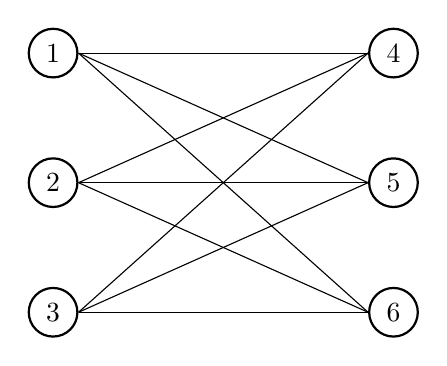
\begin{tikzpicture}[roundnode/.style={circle, draw=black!100, thick, minimum size=1mm}]

%Nodes
\node[roundnode] (circle1) {1};
\node[roundnode] (circle2) [below=of circle1] {2};
\node[roundnode] (circle3) [below=of circle2] {3};
\node[roundnode] (circle4) [right=4cm] {4};
\node[roundnode] (circle5) [below=of circle4] {5};
\node[roundnode] (circle6) [below=of circle5] {6};

%line
\draw[-] (circle1.east) -- (circle4.west);
\draw[-] (circle1.east) -- (circle5.west);
\draw[-] (circle1.east) -- (circle6.west);

\draw[-] (circle2.east) -- (circle4.west);
\draw[-] (circle2.east) -- (circle5.west);
\draw[-] (circle2.east) -- (circle6.west);

\draw[-] (circle3.east) -- (circle4.west);
\draw[-] (circle3.east) -- (circle5.west);
\draw[-] (circle3.east) -- (circle6.west);

\end{tikzpicture}
\end{center}

G = (V,E) for any order 

G = \{\{1, 2, 3, 4, 5, 6\},\{(1, 4), (1, 5), (1, 6), (2, 4), (2, 5), (2, 6), (3, 4), (3, 5), (3,6)\}

\end{enumerate}
\end{document} 
